\section{NP completeness of the Minecraft Water Problem}


\subsection{SAT $\leq_p$ MCWATER}
To encode a SAT formula $F$ in CNF with $n$ variables and $m$ clauses into an MCWATER world $W$, we define the following structures as "building blocks" of our world:



\paragraph{Input}
Each input structure represents a single boolean variable. A lapis block allows for the placement of a water source, which represents the variable's assignment. If water is placed, the corresponding boolean variable is true, while a lack of water represents false.\newline To simplify the rest of the formula construction, we designed the input structure to have two output streams, one for the current variable assignment (Fig \ref{fig:input} left) and one for the negation of that assignment (Fig \ref{fig:input} right). The negation is accomplished by using a constant water source in the not-lane, which is cut off if water is placed on the lapis block and destroys a string holding up some sand. In boolean terms, an Input represents a variable $x$ and the outputs are the literals $x$ and $\neg \; x$. An Input has a width of 6, a height of 4 and a length 6 blocks.

\begin{figure}[ht]
    \centering
    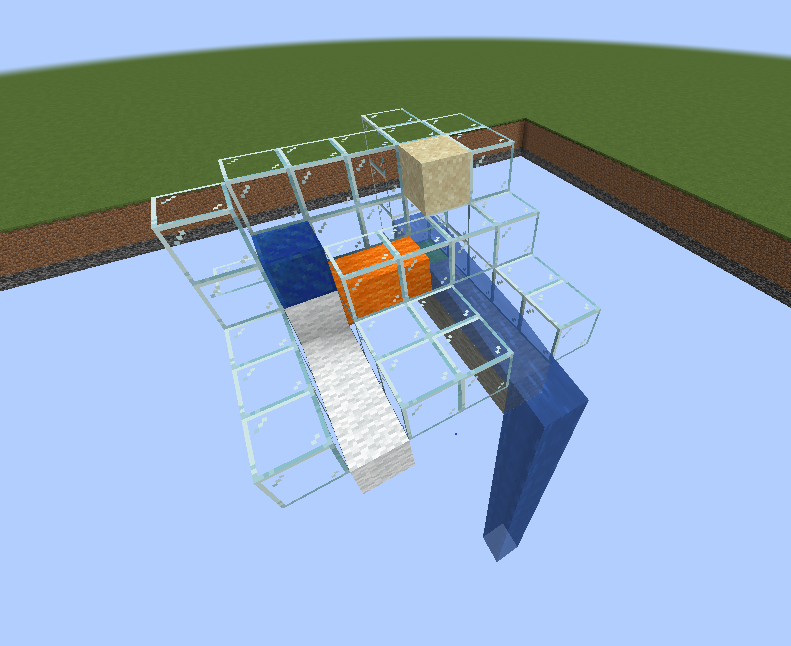
\includegraphics[width=0.5\linewidth]{images/input.png}
    \caption{A single input structure floating in the world}
    \label{fig:input}
\end{figure}



\paragraph{Splitter} \label{splitter}
Splitters represent literals in a clause and always belong to  exactly one clause and one variable of the CNF formula. They are placed sequentially after each other, starting from an input. One of their tasks is simply to provide a constant downward path to extend the streams. The other task is to split one of the streams into two when necessary. This is accomplished by removing one of the magenta blocks, which effectively creates a new stream that falls directly down. Removing the left block splits off the variable assignment, while removing the right block splits off the negated variable assignment and lets it flow into a collector for a clause.\newline In Boolean terms, this represents inserting a literal $x$ or $\neg \; x$ into a clause.\newline A Splitter has a width of 6, a height of 3 and a length of 2 blocks.

\begin{figure}[h]
    \centering
    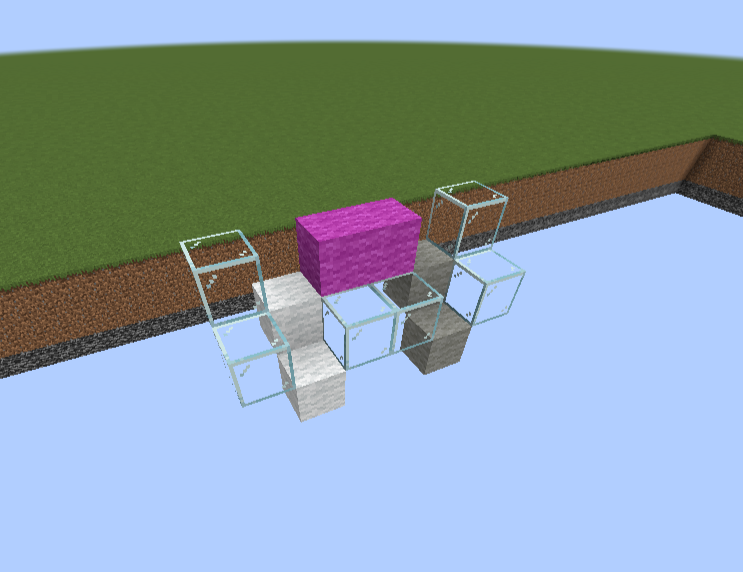
\includegraphics[width=0.5\linewidth]{images/splitter.png}
    \caption{A single splitter structure floating in the world}
    \label{fig:splitter}
\end{figure}

\pagebreak
    
\paragraph{Collector} \label{collector}
Collectors represents clauses of the CNF formulas are placed under Splitters to catch the falling streams. They are placed sequentially after each other, each time replacing the gold block at the end and effectively making sure, that it is always at the end of the chain. Like the splitters, they provide a constant down-hill to extend the streams. They also combine the outputs of the splitters and therefore act as an OR gate. The gold at the end will be covered in water if and only if one or more of the splitters output water onto the Collector chain. In boolean terms, the paths represent clauses of literals and the gold blocks at the end together with the \textbf{MCWATER} definition represent a conjunction of clauses.\newline A Collector has a width of 6, a height of 2 and a length 3 blocks.

\begin{figure}[h]
    \centering
    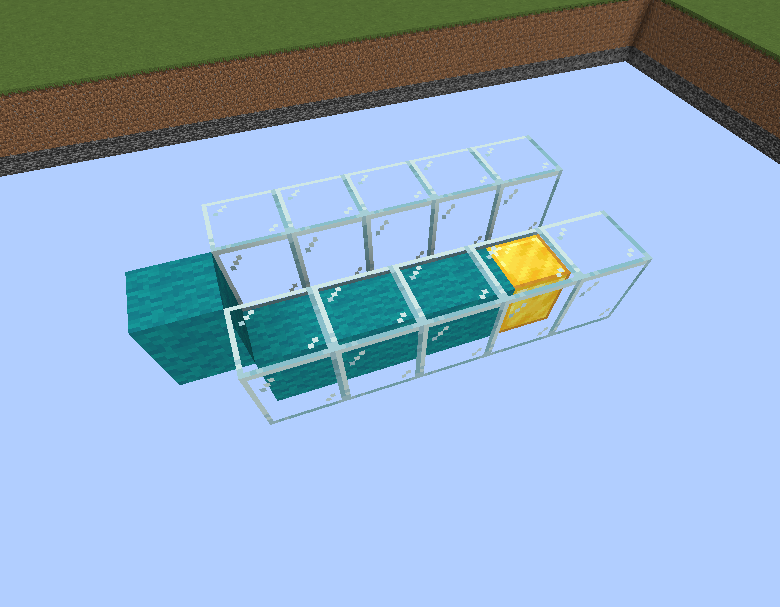
\includegraphics[width=0.5\linewidth]{images/collector.png}
    \caption{A single collector structure floating in the world}
    \label{fig:collector}
\end{figure}


\begin{figure}[h]
\centering
\begin{subfigure}{.33\textwidth}
  \centering
  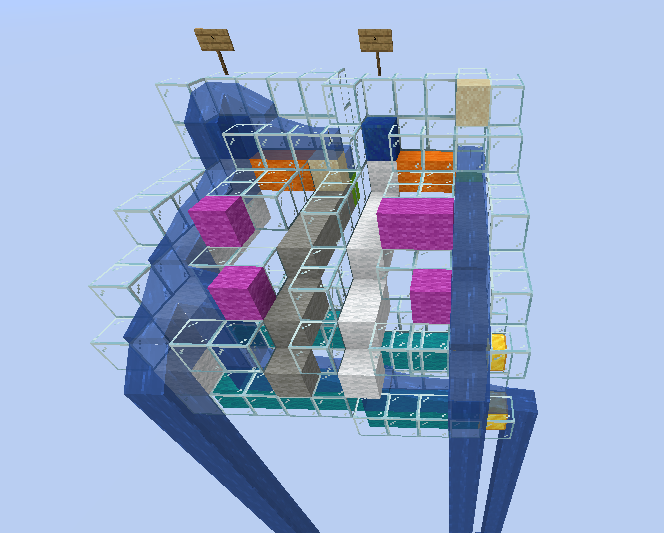
\includegraphics[width=.9\linewidth]{images/small_example_front.png}
  %\caption{A subfigure}
  %\label{fig:ex-sub1}
\end{subfigure}%
\begin{subfigure}{.33\textwidth}
  \centering
  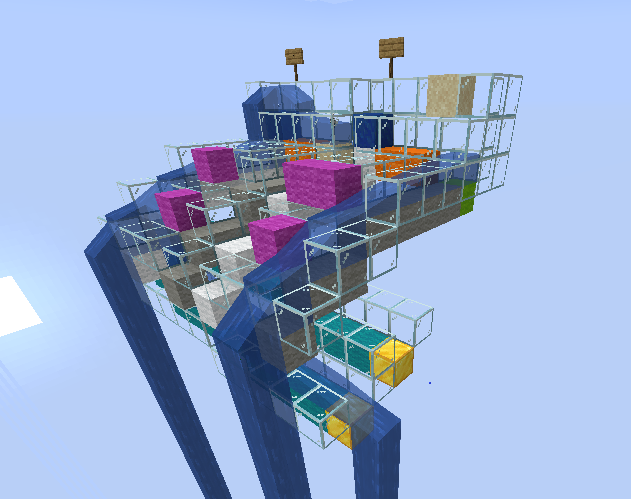
\includegraphics[width=.9\linewidth]{images/small_example_angle.png}
  %\caption{A subfigure}
  %\label{fig:ex-sub2}
\end{subfigure}
\begin{subfigure}{.33\textwidth}
  \centering
  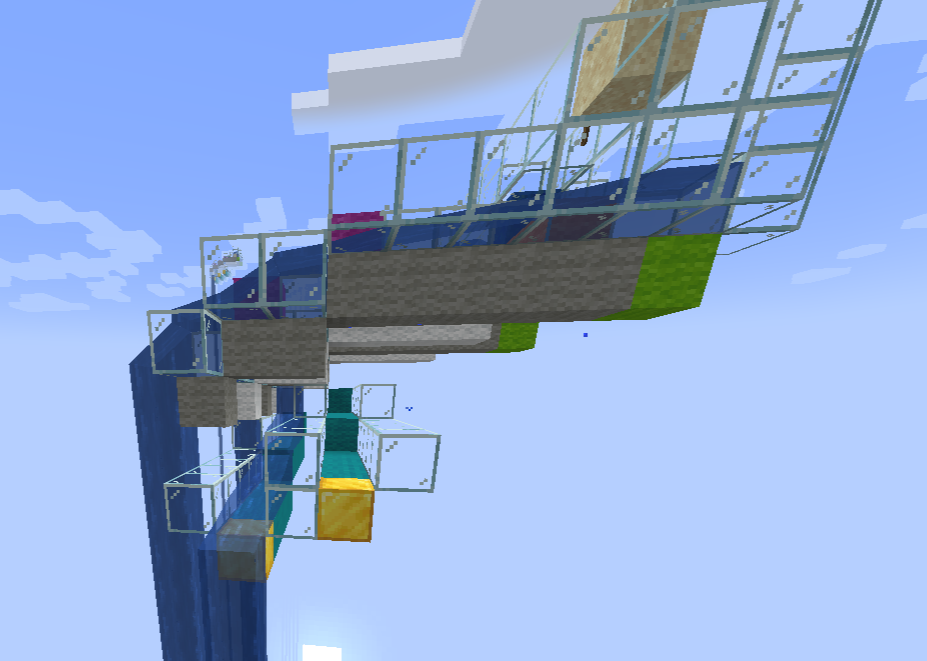
\includegraphics[width=.9\linewidth]{images/small_example_side.png}
  %\caption{A subfigure}
  %\label{fig:ex-sub2}
\end{subfigure}
\caption{A small example of a SAT formula encoded as a MCWATER world. Specifically, we show the formula $(x \vee y) \wedge (\neg \; x)$ with the assignment $x = \top, y = \bot$. The stream of variable $x$ is on the left, $y$ is on the right. The clause $(\neg \; x)$ is closest to the Inputs. Note that not all gold blocks are covered in water, because the clause $(\neg \; x)$ is not satisfied.}
\label{fig:small-example}
\end{figure}



\paragraph{Construction} \label{npcomplete:construction}
First of all, we place an input for every variable in $F$, sequentially in a row on the x-axis, where every input overlaps itself by one block with the last one.
\newline\noindent Next, we place $m$ Splitters in front of each input on the z-axis. The first Splitter is placed one y-level below the input and each following Splitter is also placed one y-level below it's predecessor, to ensure the water will always continue flowing. Additionally, if the Splitters variable is contained  as a literal in the clause, the left magenta block is removed and if the negation of the variable is contained  as a literal in the clause, the right magenta block is removed.
\linebreak

\noindent Below each Splitter, we also place a Collector starting on the block behind them on the z-axis. The leftmost Collectors will be placed 2 y-levels below the corresponding splitter, the other Collectors will always be one y-level below it's left neighbor. This is also done, to ensure a waterflow until the end. Furthermore, the Collectors overlap by one block on the x-axis. This way, the gold block of the Collectors with a right neighbor will be destroyed during the construction process and there is only exactly one gold block at the end of each Collector row.
\linebreak

\noindent Figure \ref{fig:small-example} show the result of this construction process. An assignment is already placed there, to illustrate how the individual building blocks work together to produce a final output.



\paragraph{Space Complexity}
This construction process yields a world width (x-axis) of $5 * n + 1$ (length of $n$ overlapping Inputs), length (z-axis) of $6 + 2 * m$ (length of an Input + length of $m$ Splitters) and a world height (y-axis) of $4 + m + n + 1$ (height of an Input + offsets of Splitters + offsets of Collectors + additional constant height of first collector). This results in a total world size of $(5 * n + 1) * (4 + m + n + 1) * (4 + 2m + 1) = 10m^2n + 10mn^2 + 2m^2 + 25n^2 + 77mn + 15m + 130n + 25$ blocks. It is clear to see, that the size of the resulting world $W$ is at most polynomially dependent on the size of input formula $F$.



\paragraph{Time Complexity}
To construct the world $W$ for a given formula $F$ with $n$ variables and $m$ clauses, we need to place $n$ Inputs, $n * m$ Splitters and $n * m$ Collectors. One Input needs at most $6 * 4 * 6 = 144$ block placements, one Splitter needs at most $6 * 3 * 2 + 2 = 38$ block placements (extra two because of the potential removal of the magenta blocks) and one Collector needs at most $6 * 2 * 3 = 36$ block placements.
Starting from an empty world, this yields $144n + 38mn + 36mn = 144n + 74mn$ block placements in total, which is clearly at most polynomially dependent on the size of input formula $F$.


\pagebreak

\paragraph{Equality}
The relation $x \in$ SAT if and only if $f(x) \in$ \textbf{MCWATER} is immediately obvious from our construction. For each variable in the formula we have an Input and a sequence of Splitters which deposit the variable or its negation to any clauses where they occur. For each clause, there are Collectors which combine the literals received from the Splitters. The output of these Collectors is the OR of the literals, which then flows onto single gold blocks. Per the MCWATER definition, a world is only accepted if there is a water source assignment, such that all gold blocks are covered in water. This rule plays the part of the AND for our individual collector outputs.
\linebreak

\noindent As can be seen, the constructed MCWATER world directly emulates the given SAT formula, from the individual literals to the construction and combination of clauses. Therefore, any model of the formula in SAT directly corresponds to a model in the MCWATER world and vice versa.



\subsection{3-SAT $\leq_p$ SAT}
To also show the reduction from 3-SAT, we will use the intermediate reduction to SAT, the language of satisfiable boolean formulas in CNF.\newline This relation is immediately obvious, as 3-SAT $\subset$ SAT.\newline For the Karp reduction we have $f(x) = x$ and $x \in$ 3-SAT if and only if $f(x) \in$ SAT.



\subsection{3-SAT $\leq_p$ MCWATER}
Due to the transitivity of Karp reductions, we can combine the previous reductions\newline 3-SAT $\leq_p$ SAT and SAT $\leq_p$ MCWATER to conclude 3-SAT $\leq_p$ MCWATER.



\subsection{NP-hard and NP-complete}
As shown, an arbitrary formula in 3-SAT can be converted to a world in MCWATER in polynomial time and space. This proves that MCWATER is NP-hard.\newline Given that we have found NP-hard MCWATER, we might even consider it mcICE.
\linebreak
\noindent Together with the finding that MCWATER is in NP, we have proven that MCWATER is NP-complete.

